\def \currentAuthor {Gabi Sorglos} %so kann jederzeit der Autor geändert werden -> wird in der Fusszeile angezeigt.

\chapter*{Einleitende Bemerkungen}

\chapter*{Notationen}
Beschreibung wie Code, Hinweise, Zitate etc. formatiert werden  


\chapter{Projektmanagement}
%todo: Projektmanagementscheiße bullshitten
\section{Metainformationen}
\subsection{Team}
\subsection{Betreuer}
\subsection{Partner}
\subsection{Ansprechpartner}
\section{Vorerhebungen}
\subsection{Projektzieleplan}


\newpage
\subsection{Projektumfeld}
\begin{itemize}
	\item Identifikation der Stakeholder
	\item Charakterisierung der Stakeholder
	\item Maßnahmen
	\item Grafische Darstellung des Umfeldes
\end{itemize}
\subsection{Risikoanalyse}
\subsubsection{Risikoidentifikation}
Folgende Risiken können während der Projektdurchführung erwartet werden:
\begin{itemize}
	\item[\textbf{R1}] Projektmitglied steig aus dem Projekt aus.
	\item[\textbf{R2}] Projektpartner stellt seine Kooperation ein.
	\item[\textbf{R3}] Projektpartner ändert seine Anforderungen.
	\item[\textbf{R4}] Termine können nicht eingehalten werden.
	\item[\textbf{R5}] Anforderungen werden nicht erreicht.			
\end{itemize}

\subsubsection{Bewertung und Behandlung}
Die aufgelisteten Risiken werden nach Auswirkung und Eintrittswahrscheinlichkeit bewertet.
Je höher die Zahl in der Tabelle, desto höher ist die Auswirkung bzw. Einwirkung.
\begin{table}[h]
	\begin{tabular}{l|c|c}
		\textbf{Risiko}                           & \multicolumn{1}{l|}{\textbf{Wahrscheinlichkeit}} & \multicolumn{1}{l}{\textbf{Auswirkung}} \\ \hline
		\textbf{R1} Ausstieg Projektmitglied                  & 3                                                & 10                                      \\
		\textbf{R2} Projektpartner stellt Kooperation ein     & 2                                                & 10                                      \\
		\textbf{R3} Projektpartner ändert seine Anforderungen & 4                                                & 7                                       \\
		\textbf{R4} Termine können nicht eingehalten werden   & 3                                                & 6                                       \\
		\textbf{R5} Anforderungen werden nicht erreicht       & 2                                                & 8                                      
	\end{tabular}
	\caption{Analyse Einwirkung \& Auswirkung}
	\label{Abb_Einwirkung_Auswirkung}
\end{table}
\newpage

\subsubsection{Risikomatrix}
\begin{figure}[h]
	\centering
	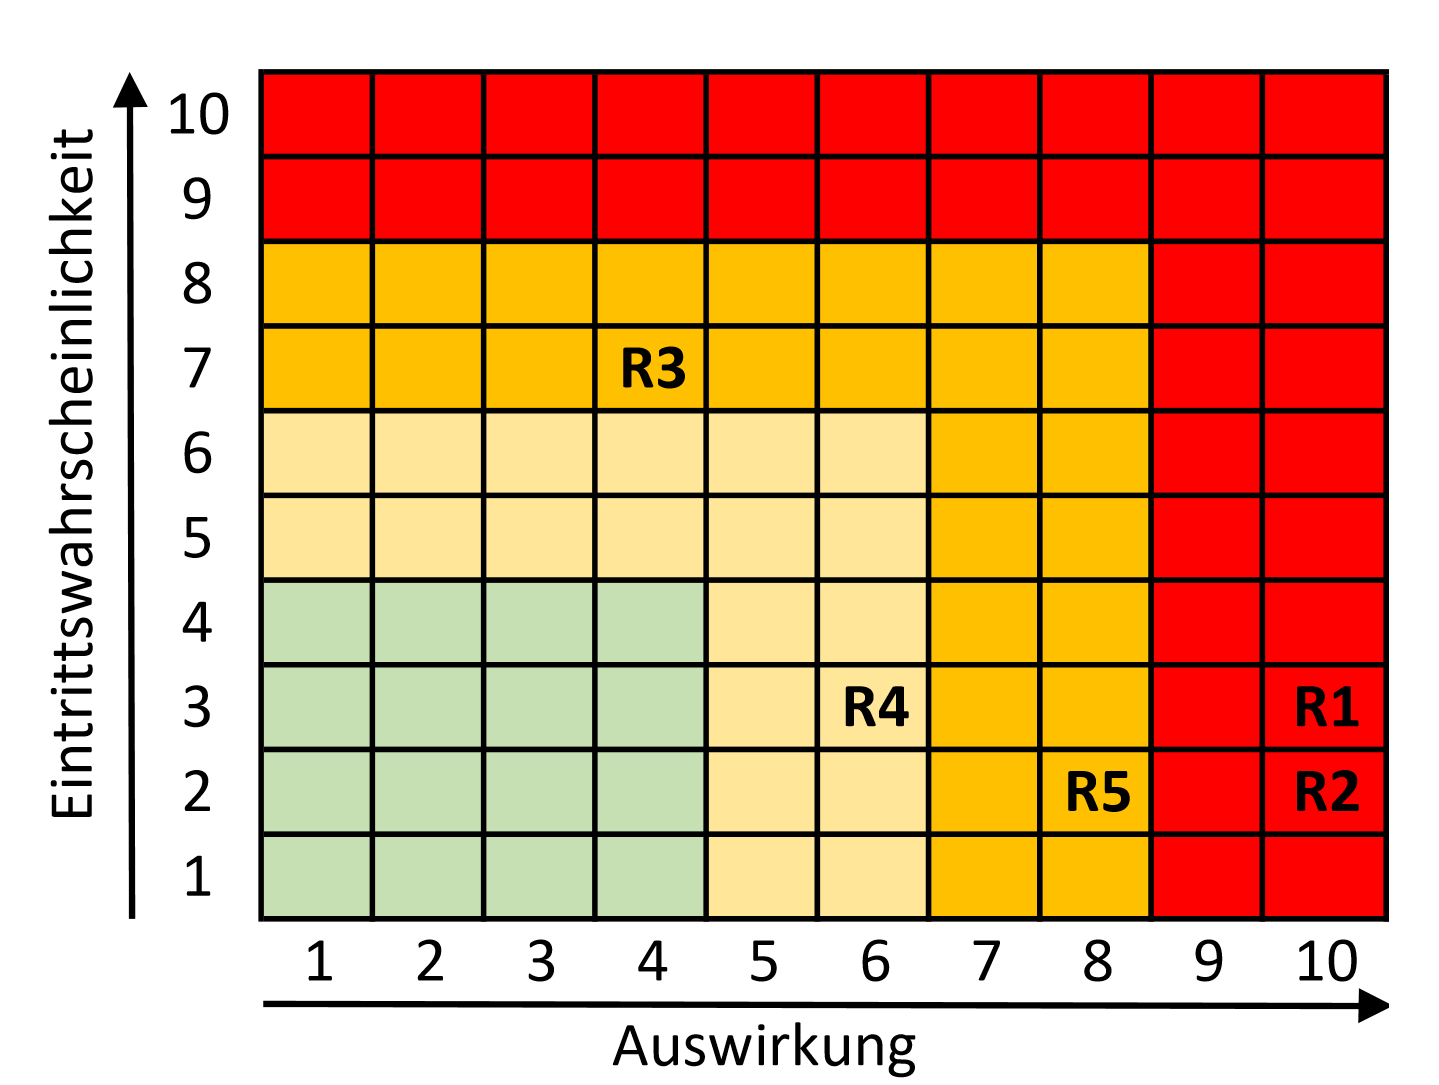
\includegraphics[scale=0.6]{figures/matrix.png}
	\caption{Risikomatrix}
	\label{Abb_Risikomatrix}
\end{figure}


\newpage
\section{Pflichtenheft}
\subsection{Zielbestimmung}
\section{IST Zustand}
IT-ManagerInnen an Tirols Schulen können Probleme mit der Infrastruktur melden und Anfragen zur Beschaffung von Ressourcen/Komponenten stellen.
\\
Sie können den Bearbeitungsverlauf ihrer Tickets beobachten. SystembetreuerInnen empfangen die Tickets der IT-ManagerInnen, welche sich in ihrem Cluster befinden. SystembetreuerInnen bearbeiten die Tickets und antworten auf die Anfragen.

\begin{figure}[h]
	\centering
	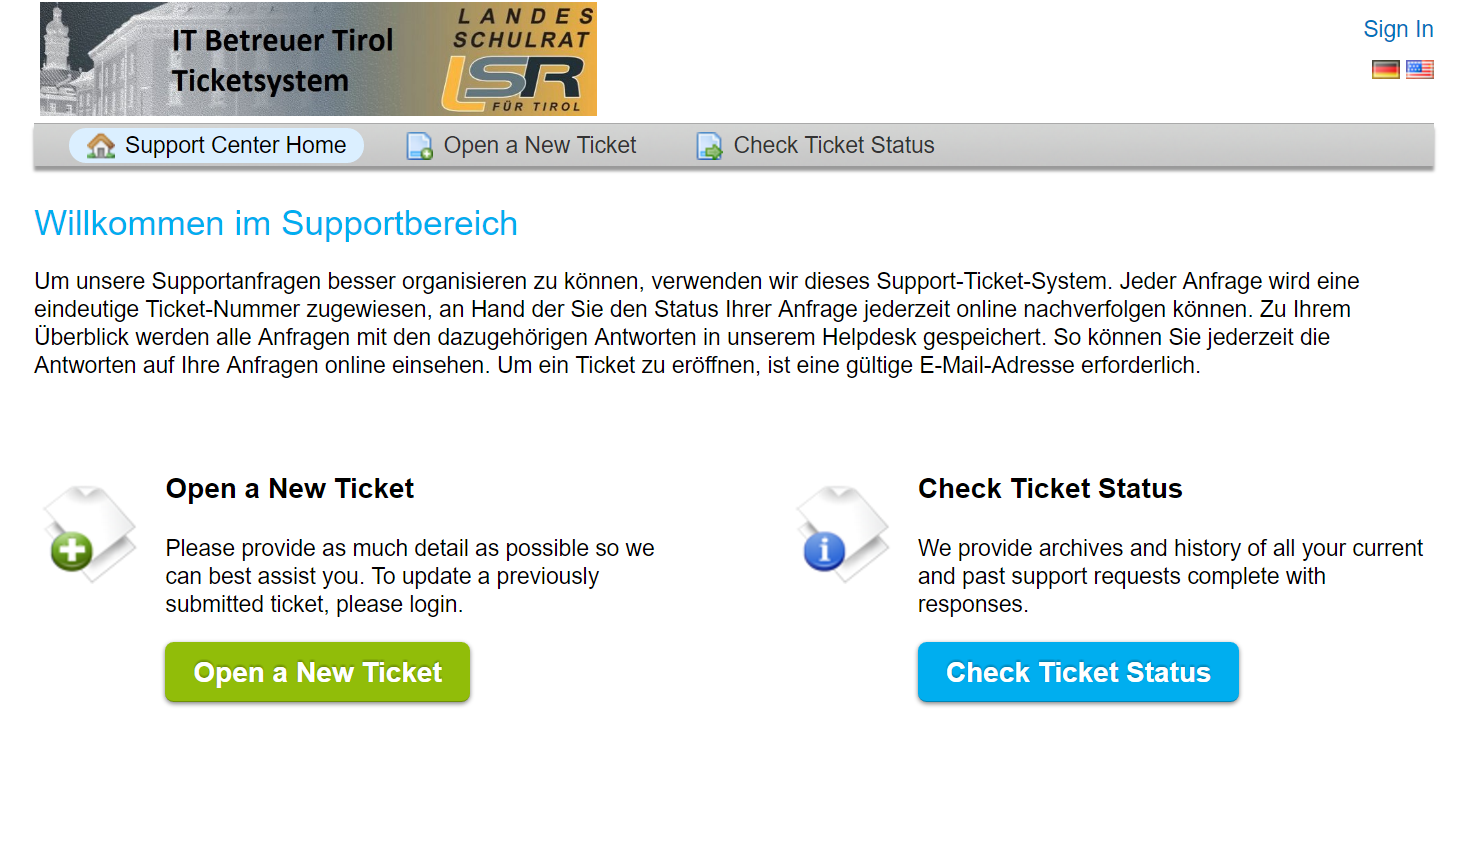
\includegraphics[scale=0.725]{figures/Ist_Login.png}
	\caption{IST-Zustand OS-Ticket}
	\label{Abb_IST-Zustand}
\end{figure}
\noindent Die Benutzerschnittstelle ist derzeit nur auf die Benutzung mit großen Bildschirmen (ab 1024 Pixel Bildschirmbreite) ausgelegt. Sie kann sich nicht an kleinere Formate (Smartphone, etc.) anpassen.

\section{SOLL Zustand}
Bessere Usability soll mit Hilfe von Mobile-First Orientierung auf Basis von Bootstrap erreicht und wenn möglich die Ticketerstellung vereinfacht werden.
\\
Das Backend soll die Aufteilung in mehrere hierarchische Organisationseinheiten ermöglichen und eine Erweiterung von Landesebene auf Bundesebene zulassen. Des Weiteren gilt es, den AnwenderInnen den Ticketingprozess intuitiver zu gestalten.

\subsection{SMART}
\begin{description}
	\item[S] Spezifisch\newline
	Systembetreuer und IT-Manager können Support- und Beschaffungsanfragen mit Hilfe des Ticketsystems abwickeln.
	\item[M] Messbar\newline
	Systembetreuer empfangen die Tickets und kümmern sich um die Probleme. Die Schulen werden in Cluster eingeteilt und von Systembetreuern verwaltet. 
	\item[A] Attraktiv\newline
	Die Plattform muss auf jedem Endgerät verfügbar sein (Responsive Design). Das Absetzen und Ansehen von Tickets soll vereinfacht werden, die Plattform bietet einige Funktionen die für das System relevant sind.
	\item[R] Realisierbar\newline
	Zum Realisieren wird eine Testumgebung von Seiten des Betreuers zur Verfügung gestellt. Das Responsive Design wird mithilfe eines Framework (Bootstrap) realisiert.
	\item[T] Terminisierbar\newline
	Im Juni 2017 wird das Projekt abgeschlossen und eine technische Dokumentation des Projekts liegt vor.
\end{description}


\subsection{Produkteinsatz und Umgebung}
%--------------------------------
%todo: Anwender des Systems beschreiben (steht auch so in der Vorlage)
%--------------------------------
\subsection{Projektumfeldanalyse}
\subsubsection{Einflussfaktoren}
Das Projekt wurde durch den Landesschulrat Tirol in Auftrag gegeben. Die Ansprechperson, Herr Helmut Hammerl, informiert uns über den IST und SOLL-Zustand der Plattform und unterstützt das Projekt mit Ideen und Hilfestellungen bei Problemstellungen.
\\
Des Weiteren beeinflussen die Anwender (IT-Manager) und die Systembetreuer der Plattform das Projektresultat. Da auf die Anwenderfreundlichkeit viel Wert gelegt wird, spielen diese Faktoren eine wirkliche Rolle.
\\
Die Projektbetreuer Stefan Stolz und Alexander Scharmer sind für auftretende Fragen, bezüglich Problemstellungen die während des Projekts auftreten können, enorm einflussreich.
\newpage
\subsection{Stakeholder}
\subsubsection{Stakeholder Identifizieren}
\begin{table}[h]
	\centering
	\begin{tabular}{|lll|}
		\hline
		Stakeholder          & Einfluss &  Konfliktpotential      \\ \hline                         
		Mag. Helmut Hammerle & 3         & 0                  \\ 
		Dr. Stefan Walch     & 2         & 0                  \\
		Stefan Stolz         & 1         & +                  \\ 
		Alexander Scharmer   & 1         & +                  \\ 
		Michael Gamper       & 0         & 0                  \\ 
		LSI DI Anton Lendl   & 3         & 0                  \\ 
		Team Mitglieder      & 2         & 0                   \\ \hline			
	\end{tabular}
	\caption{Stakeholder Identifikation}
	\label{Tbl_Stakeholder_Identifikation}
\end{table}


\subsubsection{Stakehnolder Klassifizieren}	

%todo: Formatierung der Tabelle
\begin{table}[h]
	\centering
	\begin{tabular}{|lll|}
		\hline
		Stakeholder          & Risiken durch Stakeholder                        & Strategien                                            \\ \hline
		Mag. Helmut Hammerle & Ändern der Ansprüche          & Unterschriebenes Pflichtenheft  \\
		Dr. Stefan Walch      & Nicht bestätigen des Projektantrages             & Durchdachter Projektantrag                            \\
		Stefan Stolz         & falsche Informationen, kein Interesse & regelmäßiges Treffen             \\
		Alexander Scharmer   & falsche Informationen, kein Interesse & regelmäßiges Treffen              \\
		Michael Gamper       & Nicht bestätigen des Projektantrages             & Durchdachter Projektantrag                            \\
		LSI DI Anton Lendl   & Nicht bestätigen des Projektantrages             & Durchdachter Projektantrag                            \\
		Team Mitglieder      & Mangelnde Motivation                             & Faire Arbeitsverteilung           \\ \hline			
	\end{tabular}
	\caption{Stakehodler Klassifikation}
	\label{Tbl_Stakeholder_Klassifikation}
\end{table}


\subsection{Funktionalitäten}
\subsection{Muss Anforderungen}
IT-ManagerInnen und Systembetreuer müssen sich unter itsys-tirol.at, einem Portal des Landesschulrates, basierend auf OSticket anmelden können. Des Weiteren sollen die Schulen selbst bestimmen, wer einen Zugang zum Portal erhalten soll, um Tickets erstellen zu können.
\\
Die angemeldeten IT-ManagerInnen müssen Probleme mit der Infrastruktur melden können und Anfragen zur Beschaffung von Ressourcen bzw. Komponenten einreichen können.
\\
SystembetreuerInnen müssen die Tickets der IT-ManagerInnen empfangen, welche sich in ihrem Cluster befinden. Die eingereichten Tickets sollen von den Systembetreuern bearbeitet werden können.

\subsection{Soll Anforderungen}
Es soll eine neue Weboberfläche entwickelt werden, die auf dem HTML \& CSS Framework Bootstrap basiert. Dieses soll sich auf Einfachheit in der Anwendung und Benutzerfreundlichkeit fokussieren. Die Latenzzeit sollte so niedrig wie möglich gehalten werden um ein Reibungsloses Arbeiten zu ermöglichen.

%todo: Testfälle sind furchtbar und müssen generell nocheinmal überarbeitet werden
\subsection{Testszenarien und Testfälle}
Die Testfälle in unserem Projekt beziehen sich auf das Ticketingsystem OSTicket.

\section{Testfälle}
\subsection{Testfall A}
\begin{itemize}
	\item \textbf{Beschreibung:} Ein IT-Manager möchte ein Ticket erstellen.
	\item \textbf{Vorbedingung:} Der User benötigt ein internetfähiges Gerät und muss im Portal eingeloggt sein.
	\item \textbf{Aktion:} Der Benutzer wählt den Tab "Neues Ticket" und füllt die notwendigen Felder aus.
	\item \textbf{Soll-Reaktion:} Das System setzt das Ticket für den zuständigen Systembetreuer sichtbar.
\end{itemize}
Tester:
\\M
Datum:

\subsection{Testfall B}
\begin{itemize}
	\item \textbf{Beschreibung:} Ein Systembetreuer möchte ein Ticket bearbeiten.
	\item \textbf{Vorbedingung:} Der Systembetreuer benötigt ein internetfähiges Gerät und muss im Portal eingeloggt sein.
	\item \textbf{Aktion:} Der Systembetreuer wählt den Tab "Meine Tickets" und wählt ein Ticket aus das Bearbeitet werden muss. Durch die Beschreibung des Tickets, weiß der Systembetreuer über die Problemstellung Bescheid und kann dementsprechend handeln.
	\item \textbf{Soll-Reaktion:} Der Systembetreuer kann sich um die Problemstellung kümmern und das Ticket nach erfolgreicher Bearbeitung wieder schließen.
\end{itemize}
Tester:
\\
Datum:

\subsection{Testfall C}
\begin{itemize}
	\item \textbf{Beschreibung:} Ein Anwender möchte ein bestimmtes Ticket suchen und dieses begutachten. 
	\item \textbf{Vorbedingung:} Der Anwender benötigt ein internetfähiges Gerät und muss im Portal eingeloggt sein.
	\item \textbf{Aktion:} Der Anwender gibt im Suchfeld ein Stichwort ein nach dem er suchen möchte. 
	\item \textbf{Soll-Reaktion:} Das gesuchte Ticket soll angezeigt werden.
\end{itemize}
Tester:
\\
Datum:



\subsection{Liefervereinbarung}
\begin{itemize}
	\item Lieferumfang
	\item Modus
	\item Verteilung(Deployment)
\end{itemize}

%todo: viel Bullshitten
\section{Planung}
\subsection{Projektstrukturplan}
\subsection{Meilensteine}
\subsection{Gant-Chart}
\subsection{Abnahmekriterien}
\subsection{Pläne zur Evaluierung}
\subsection{Ergänzungen und zu klärende Punkte}

\chapter{Vorstellung des Produktes}
In diesem Kapitel werden die einzelnen Ansätze aufgelistet und evaluiert, die während des Projekts durchprobiert wurden.
\section{Realisierbarkeit OSTicket}
OSTicket hat sich als umfangreicher herausgestellt wie zu Beginn des Projekts angenommen wurde. Nach Ausarbeitung des konzeptuellen Ziels des Projektes erfolgte eine lange Phase der Evaluation, Einarbeitung und Dokumentation von OSTicket. Nach ca. 30 Stunden dieser Phase, in der die Komplexität und Schwerfälligkeit des Systems OSTicket langsam zu Tage gefördert wurde. Die Anzahl der Dateien setzt sich folgendermaßen zusammen:
\begin{itemize}
	\item 414 .php Dateien
	\item 15 .css Dateien
	\item 9 .less Dateien
	\item 61 .sql Dateien
	\item 1 .html Datei
	\item \textbf{Ges. 500 Dateien}
\end{itemize}

Ein weiteres Hindernis ergibt sich durch die Absenz einer auch nur annähernd aktuellen Dokumentation des laufend erweiterten und angepassten OSTicket.
\\
Um die Realisierbarkeit zu veranschaulichen nun einige Codeauszüge aus OSTicket.
\subsection{Codebeispiele}
\begin{lstlisting}[language=PHP, caption=Auszug aus osTicket, label=code:qj]
<?php
/**************************************************
main.inc.php

Master include file which must be included at the 
start of every file.
The brain of the whole sytem. Don't monkey with it.

Peter Rotich <peter@osticket.com>
Copyright (c)  2006-2013 osTicket
http://www.osticket.com

Released under the GNU General Public License WITHOUT
 ANY WARRANTY.
See LICENSE.TXT for details.

vim: expandtab sw=4 ts=4 sts=4:
***************************************************/

#Disable direct access.
if(isset($_SERVER['SCRIPT_NAME'])
&& !strcasecmp(basename($_SERVER['SCRIPT_NAME'])
,basename(__FILE__)))
die('kwaheri rafiki!');

require('bootstrap.php');
Bootstrap::loadConfig();
Bootstrap::defineTables(TABLE_PREFIX);
Bootstrap::i18n_prep();
Bootstrap::loadCode();
Bootstrap::connect();

#Global override
$_SERVER['REMOTE_ADDR'] = osTicket::get_client_ip();

if(!($ost=osTicket::start()) || !($cfg = $ost->getConfig()))
Bootstrap::croak(__('Unable to load config info 
from DB. Get tech support.'));

//Init
$session = $ost->getSession();

//System defaults we might want to make global//
#pagenation default - user can override it!
define('DEFAULT_PAGE_LIMIT', $cfg->getPageSize()?$cfg->getPageSize():25);

#Cleanup magic quotes crap.
if(function_exists('get_magic_quotes_gpc') && get_magic_quotes_gpc()) {
$_POST=Format::strip_slashes($_POST);
$_GET=Format::strip_slashes($_GET);
$_REQUEST=Format::strip_slashes($_REQUEST);
}

// extract system messages
$errors = array();
$msg=$warn=$sysnotice='';
if ($_SESSION['::sysmsgs']) {
extract($_SESSION['::sysmsgs']);
unset($_SESSION['::sysmsgs']);
}
?>

\end{lstlisting}
%todo: Zitate (Codezitate des Programmierers, Netzer fragen)
%todo: wie genau soll man den begründen das da Code a scheiß is?
In diesem Codeauszug wird die Komplexität von osTicket sehr gut veranschaulicht, der Aufruf von elf statischen Funktionen und der dürftigen Dokumentation der Programmierer "Don't monkey around with it", machen den Code unlesbar.






%----------------------------------------------
\section{Systemdokumentation}
%todo: Systemdokumentation aus SYP hinzufügen, ist jedoch nicht ganz so einfach da Probleme mit Packages auftreten 


%-------------------------------------
%todo: Formatierungschaos im Chapter Problemanalyse beheben und Inhalt überarbeiten
%-------------------------------------

\chapter{Problemanalyse}

\section{USE-Case-Analyse}
{\linespread{.5}
	\textbf{Akteure:}
	\begin{itemize}
		\item Systembetreuer
		\item Anwender (IT-Manager und eventuell Lehrer, in Folgendem Anwender genannt)
\end{itemize}}

\vspace{-.5cm}
\begin{table}[h]
	\centering
	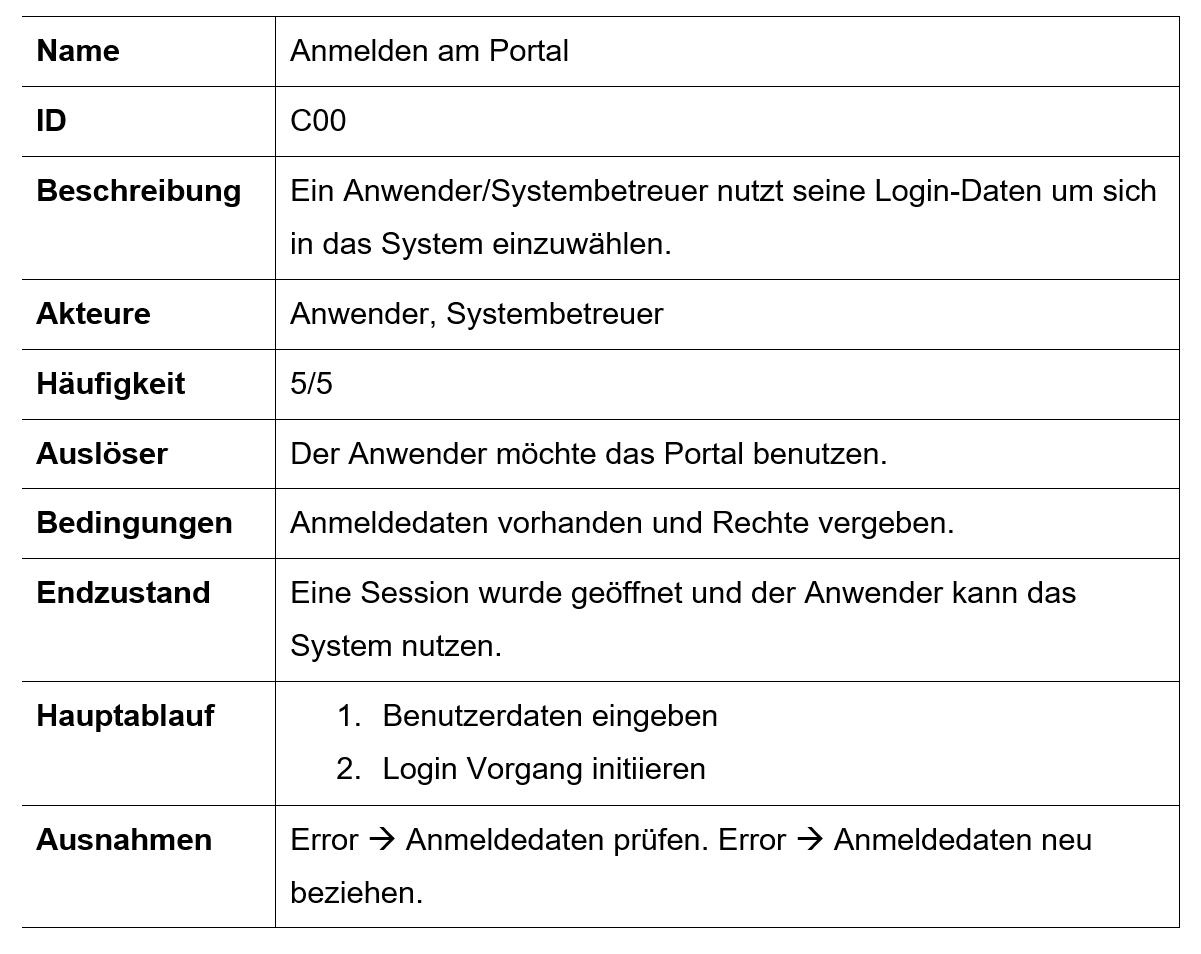
\includegraphics[scale=0.51]{figures/C00.png}
	\caption{Use-Case C00}
	\label{Abb_C00}
\end{table}
\newpage
\vspace{-.5cm}	
\begin{table}[h]
	\centering
	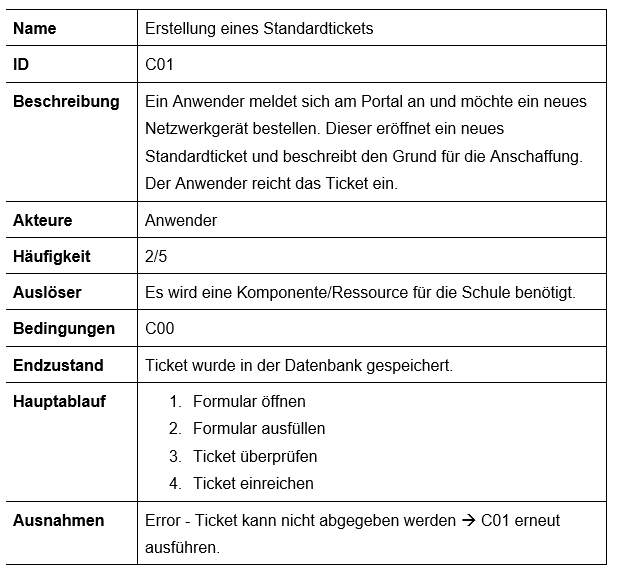
\includegraphics[scale=0.55]{figures/C01.png}
	\caption{Use-Case C01}
	\label{Abb_C01}
\end{table}
\newpage
\vspace{-.5cm}	
\begin{table}[h]
	\centering
	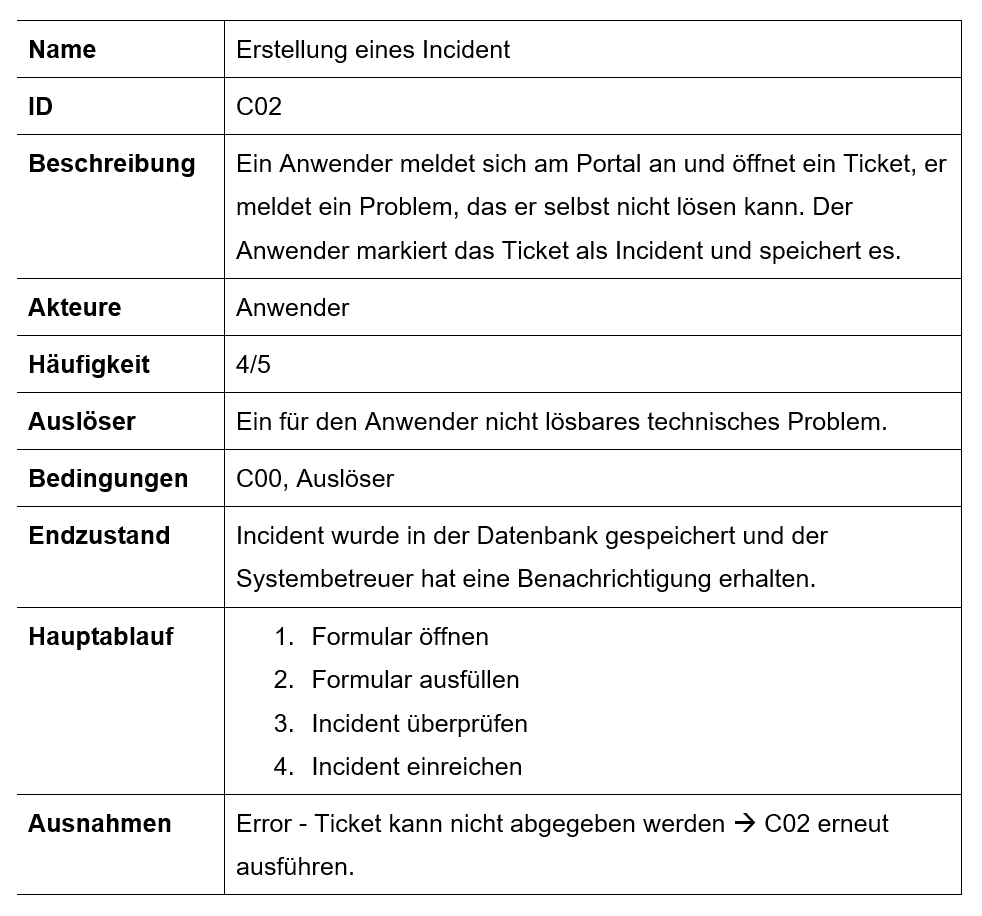
\includegraphics[scale=0.6]{figures/C02.png}
	\caption{Use-Case C02}
	\label{Abb_C02}
\end{table}

\vspace{-.5cm}	
\begin{table}[h]
	\centering
	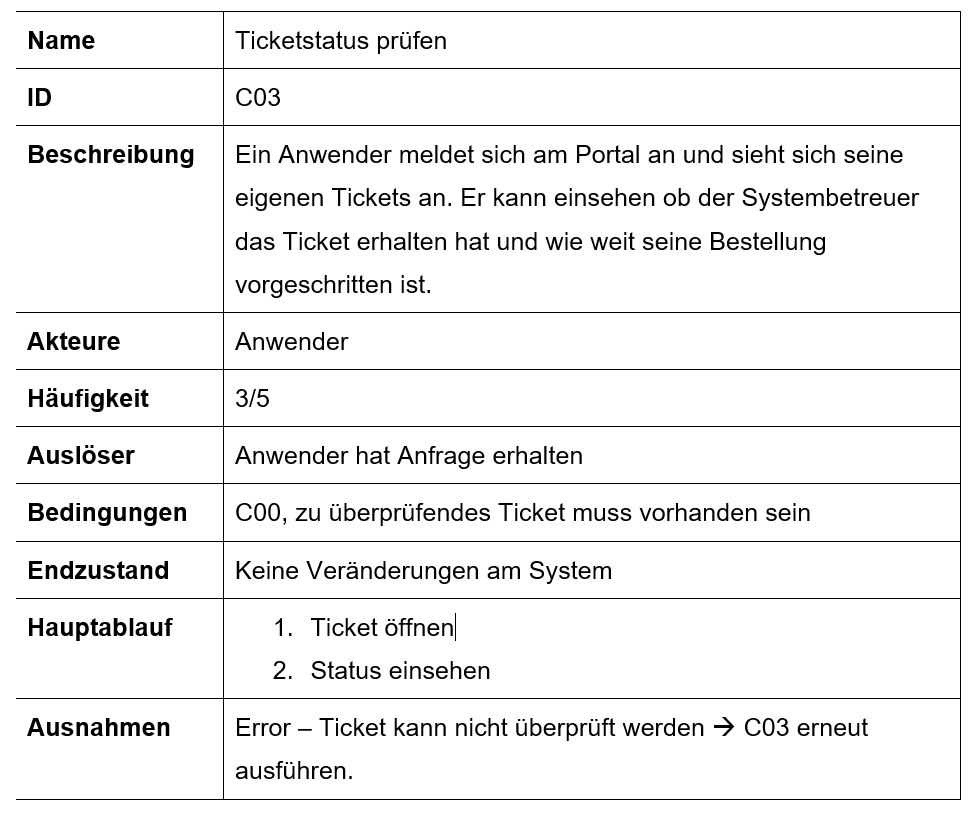
\includegraphics[scale=0.62]{figures/C03.png}
	\caption{Use-Case C03}
	\label{Abb_C03}
\end{table}
\newpage
\vspace{-.5cm}	
\begin{table}[h]
	\centering
	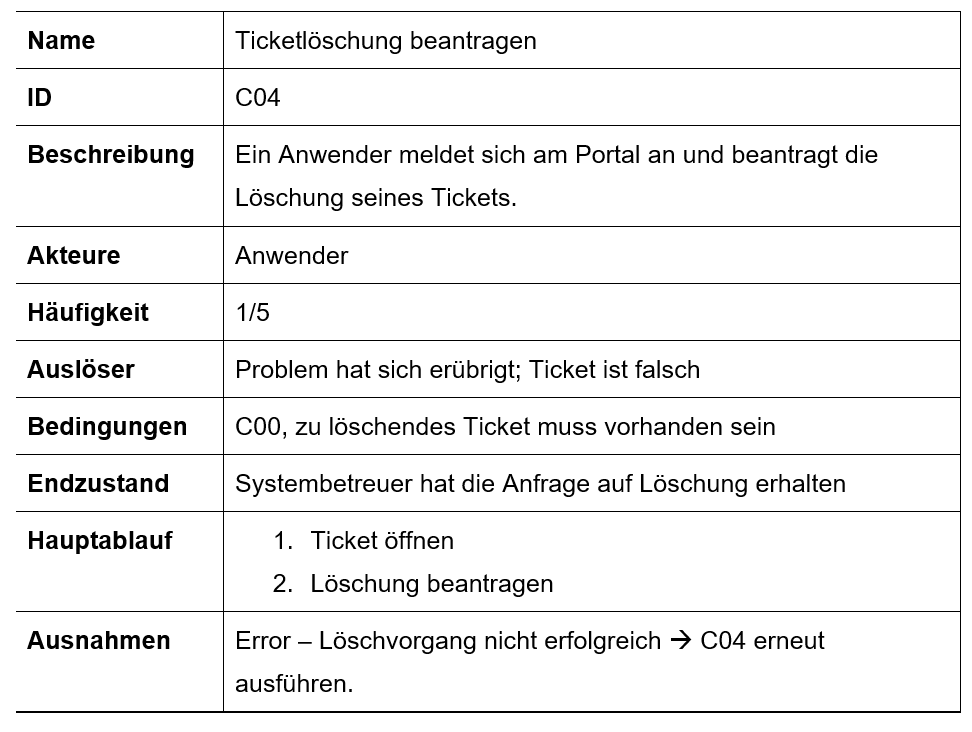
\includegraphics[scale=0.62]{figures/C04.png}
	\caption{Use-Case C04}
	\label{Abb_C04}
\end{table}


\vspace{-.5cm}	
\begin{table}[h]
	\centering
	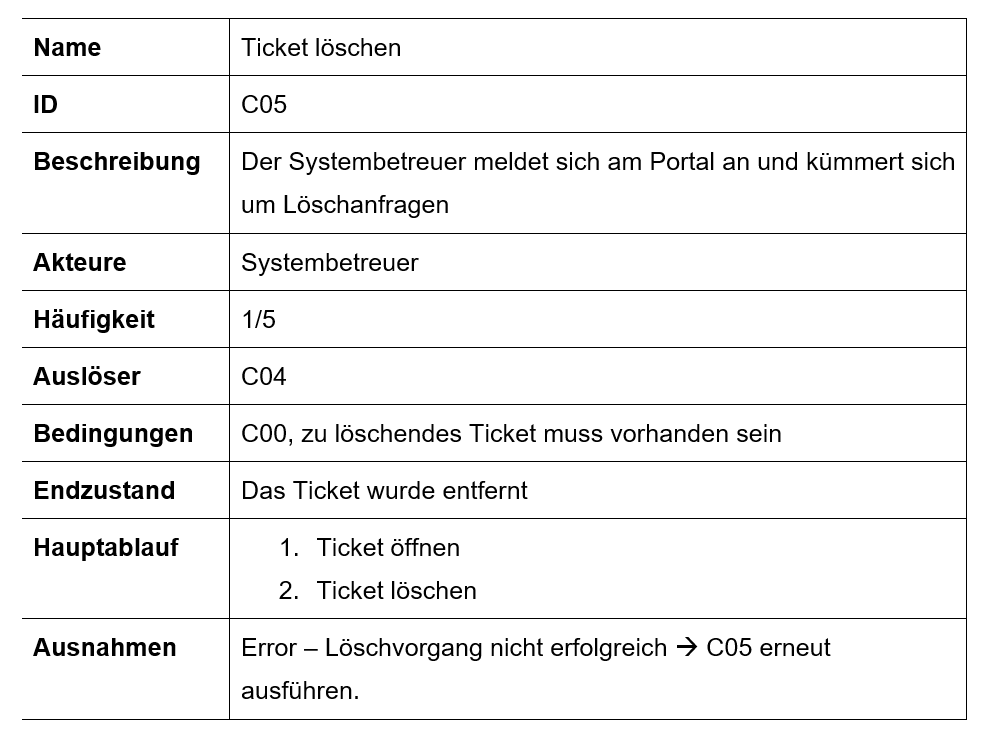
\includegraphics[scale=0.62]{figures/C05.png}
	\caption{Use-Case C05}
	\label{Abb_C05}
\end{table}
\newpage
\vspace{-.5cm}	
\begin{table}[h]
	\centering
	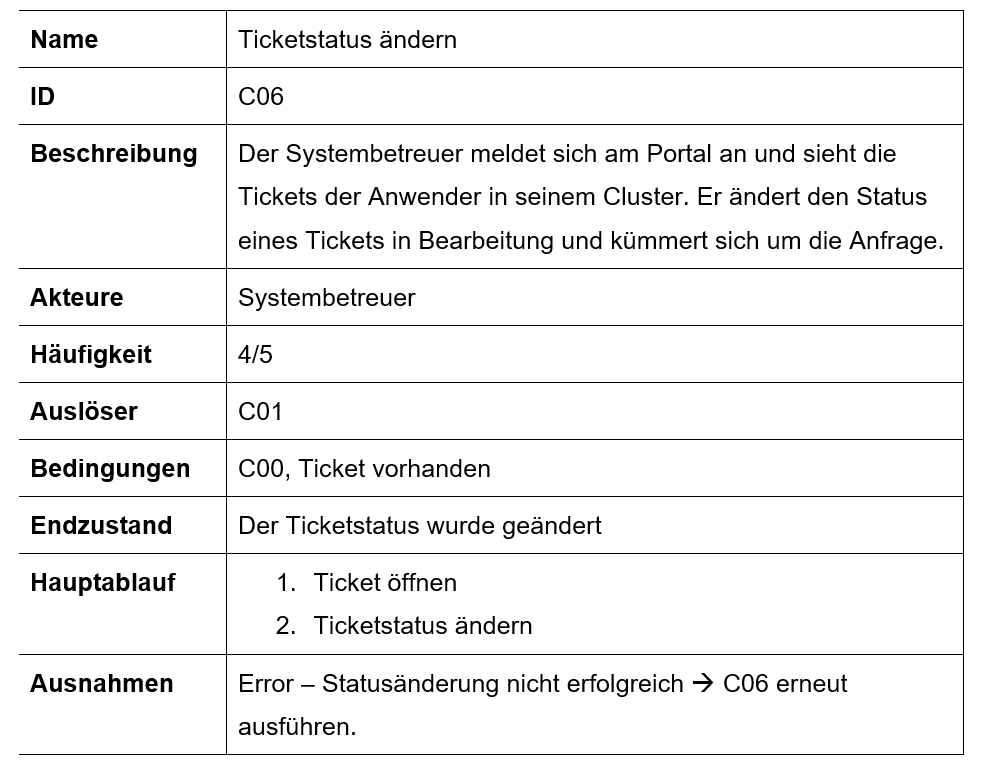
\includegraphics[scale=0.62]{figures/C06.png}
	\caption{Use-Case C06}
	\label{Abb_C06}
\end{table}
\newpage
\vspace{-.5cm}	
\begin{table}[h]
	\centering
	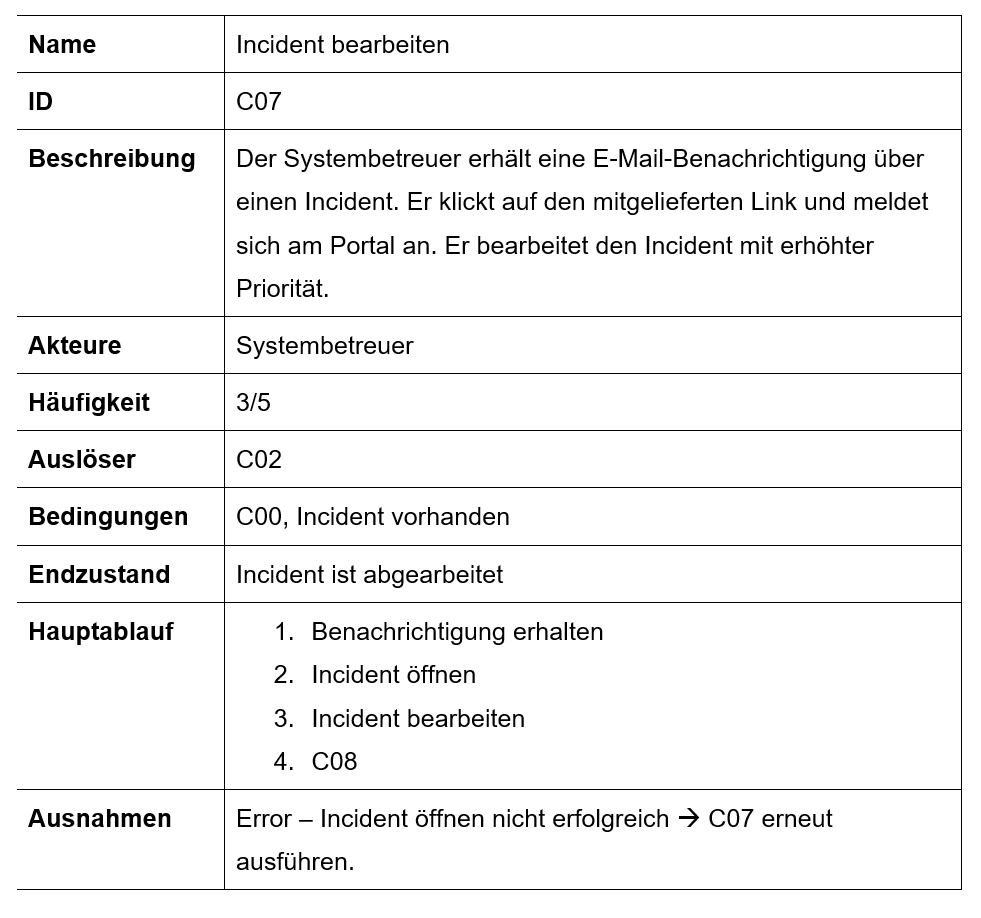
\includegraphics[scale=0.62]{figures/C07.png}
	\caption{Use-Case C07}
	\label{Abb_C07}
\end{table}

\vspace{-.5cm}	
\begin{table}[h]
	\centering
	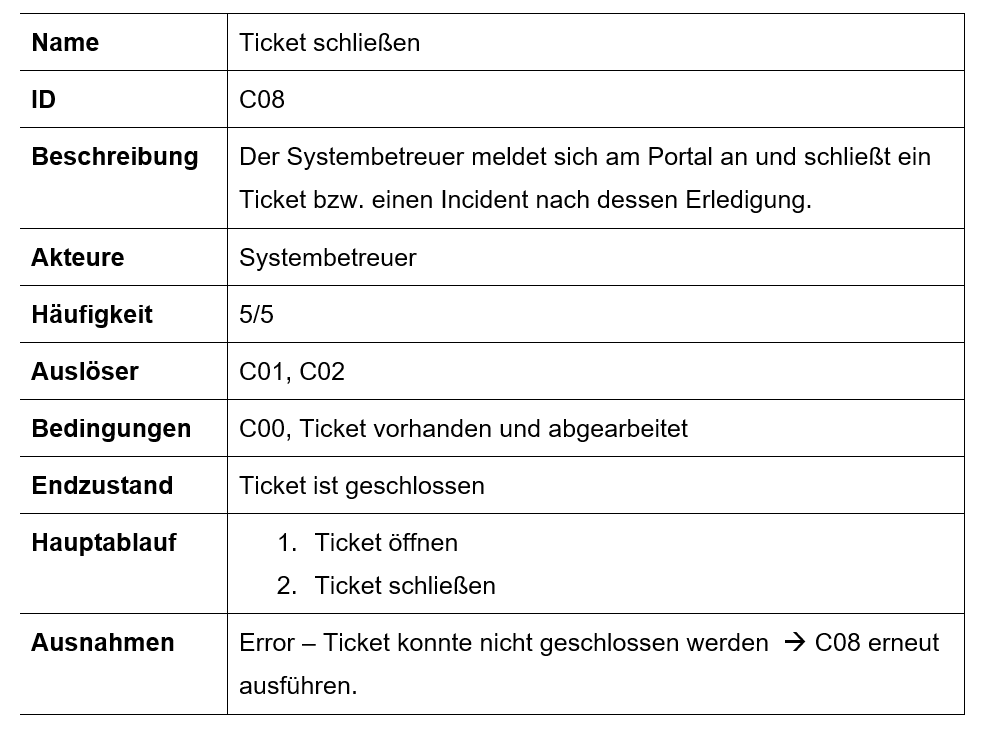
\includegraphics[scale=0.62]{figures/C08.png}
	\caption{Use-Case C08}
	\label{Abb_C08}
\end{table}


\subsection{Ablaufbeschreibung}
\textbf{C00:}
\\ 
Der Benutzer wird aufgefordert seine Benutzerdaten einzugeben.
Hat er die Daten richtig eingegeben wird er angemeldet. Sind die Daten falsch kommt er zurück zur Dateneingabe.
\\
\textbf{C01:}
\\
Der Benutzer muss zuerst ein Formular öffnen, um ein Ticket erstellen zu können. Anschließend muss das Formular ausgefüllt werden. 
\\
Nach dem Überprüfen des Tickets kann der Benutzer sich entscheiden ob er das Ticket abschickt oder ob er Änderungen vornehmen möchte. 
\\
Wenn das Abschicken fehlgeschlagen ist kommt er zum Anfang zurück. Wenn das abschicken erfolgreich war, wird das Ticket in der Datenbank gespeichert.
\\
\textbf{C02:}
\\
Der Benutzer muss zuerst ein Formular öffnen um einen Incident erstellen zu können. Anschließend muss das Formular ausgefüllt werden. Nach dem Überprüfen des Incident kann der Benutzer sich entscheiden, ob er den Incident abschickt oder ob er Änderungen vornehmen möchte.
\\
Wenn das Abschicken fehlgeschlagen ist kommt er zum Anfang zurück. Wenn das abschicken erfolgreich war wird der Incident in der Datenbank gespeichert und der Systembetreuer erhält eine Benachrichtigung.
\\
\textbf{C03:}
\\
Der Benutzer muss das Formular öffnen um den Status zu sehen. Ist das Öffnen fehlgeschlagen kommt er wieder zum Ausgangspunkt und kann es nochmal versuchen.
\\
\textbf{C04:}
\\
Um die Löschung beantragen zu können muss der Benutzer zuerst das Ticket öffnen. Danach kann er die Löschung beantragen. Schlägt dies fehl kommt er wieder zurück an den Anfang und kann es nochmal versuchen. War der Antrag auf Löschung erfolgreich erhält der Systembetreuer eine Anfrage zur Löschung.
\\
\textbf{C05:}
\\
Um ein Ticket zu löschen muss der Systembetreuer das Ticket öffnen und löschen. Schlug dies fehl kommt er wieder zurück an den Anfang und kann es nochmal versuchen. War das Löschen erfolgreich wurde das Ticket aus der Datenbank entfernt.
\\
\textbf{C06:}
\\
Um den Ticketstatus ändern zu können muss der Systembetreuer das Ticket öffnen und ändern. Schlug dies fehl kommt er wieder zurück an den Anfang und kann es nochmal versuchen. War das ändern erfolgreich wurde der Ticketstatus geändert.
\newpage
\textbf{C07:}
\\
Um ein Ticket schließen zu können muss der Systembetreuer das Ticket öffnen um es dann zu schließen. Schlug dies fehl kommt er wieder zurück an den Anfang und kann es nochmal versuchen. War das schließen erfolgreich ist das Ticket geschlossen.

\newpage
\section{Wireframes}	
\begin{figure}[h]
	\centering
	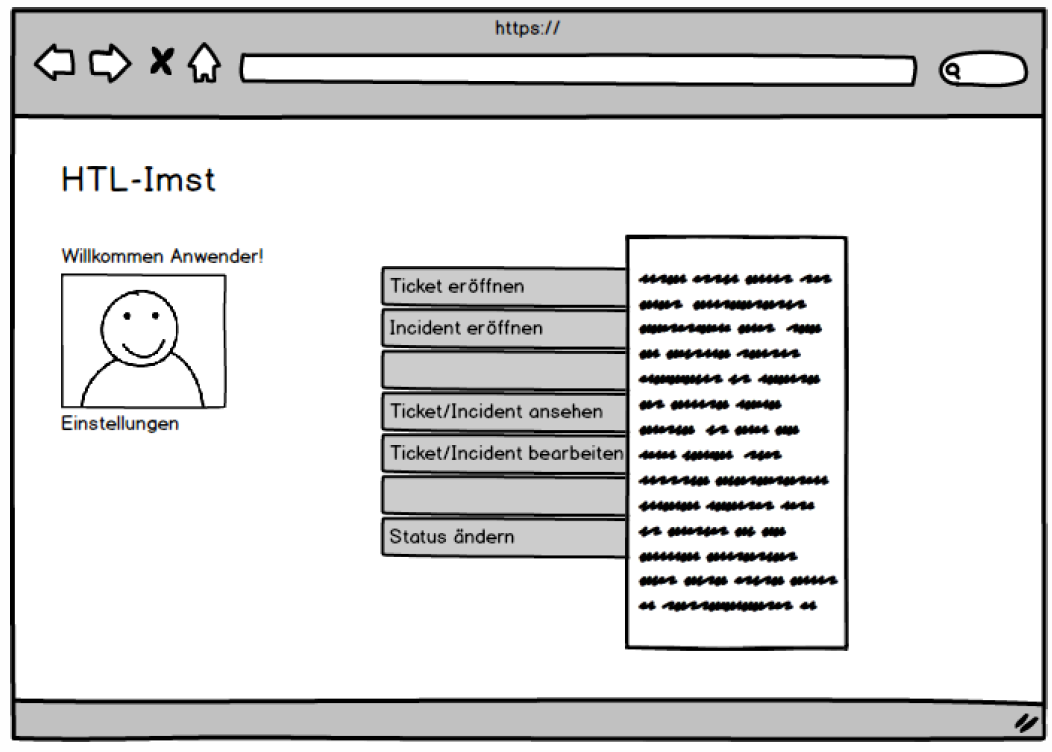
\includegraphics[scale=0.44]{figures/Wireframe_Anwender.png}
	\caption{Mockup Anwendersicht}
	\label{Abb_Mockup_Anwendersicht}
\end{figure}

\vspace{-.5cm}
\begin{figure}[h]
	\centering
	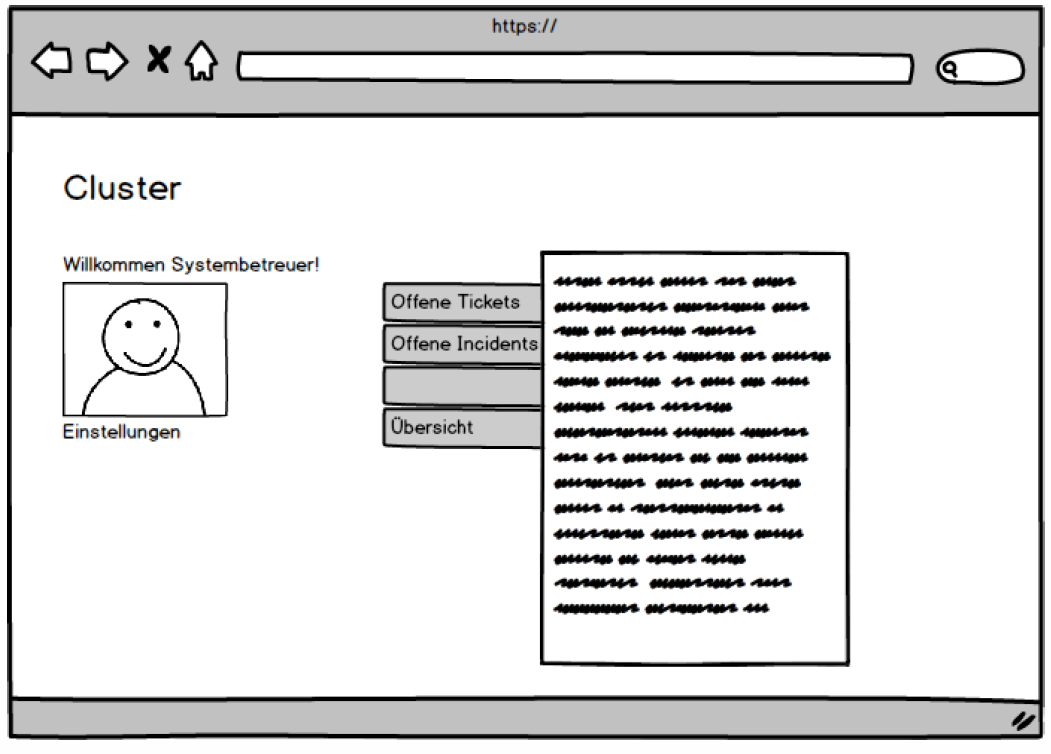
\includegraphics[scale=0.399]{figures/Wireframe_Systembetreuer.png}
	\caption{Mockup Systembetreuer}
	\label{Abb_Mockup_Systembetreuer}
\end{figure}



\vspace{.5cm}
\begin{figure}[h]
	\centering
	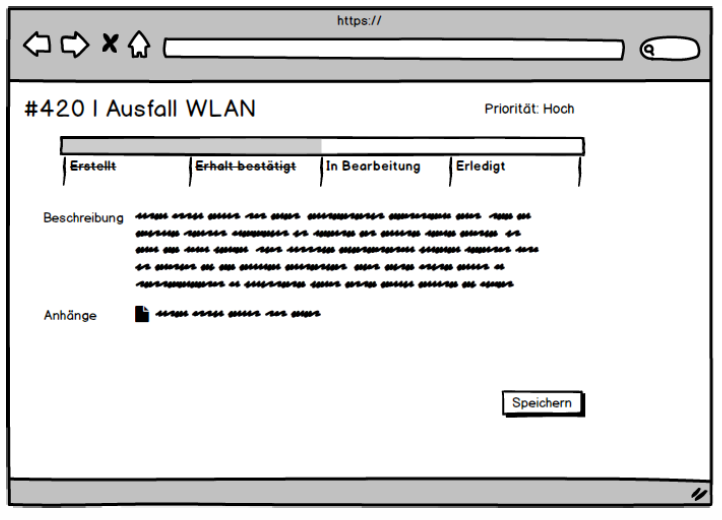
\includegraphics[scale=0.582]{figures/Wireframe_Ticket.png}
	\caption{Mockup Ticketstatus}
	\label{Abb_Mockup_Ticketstatus}
\end{figure}	

\newpage
\section{Prototyp}
\begin{figure}[h]
	\centering
	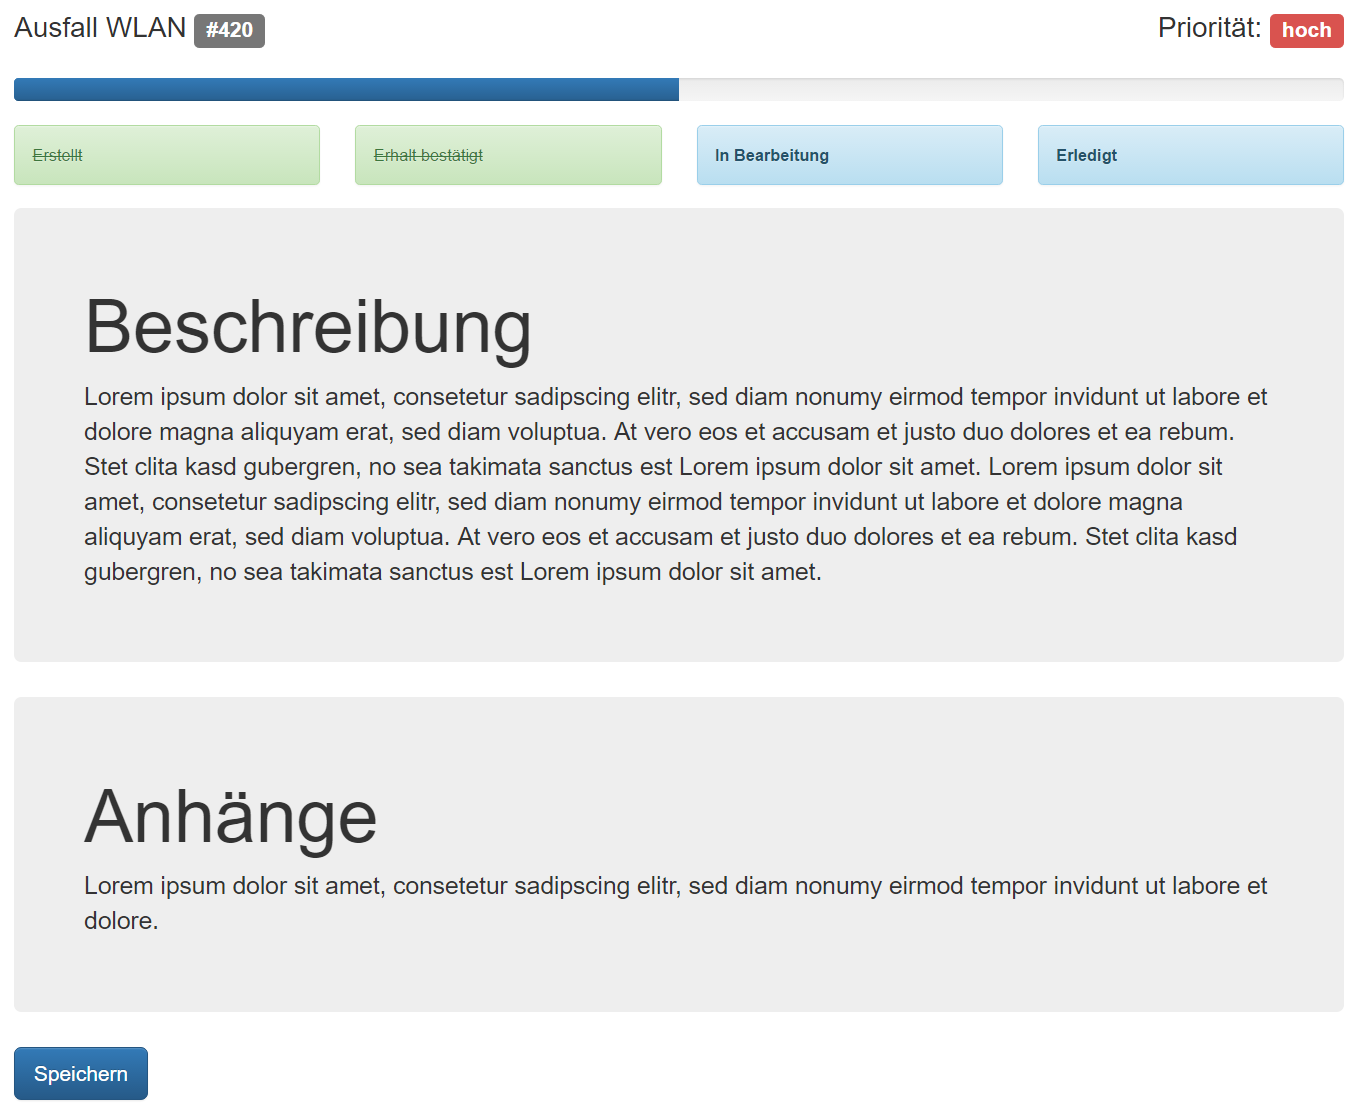
\includegraphics[scale=0.8]{figures/Prototyp.png}
	\caption{Prototyp Ticketstatus}
	\label{Abb_Prototyp_Ticketstatus}
\end{figure}


%-------------------------------------------------
%Chapter Problemanalyse Formatierungschaos bis zu diesem Punkt
%-------------------------------------------------




\newpage
\section{Domain-Class-Modelling}
\begin{itemize}
	\item "Dinge" (Rollen, Einheiten, Geräte, Events etc.) identifizieren, um die es im Projekt geht
	\item ER-Modellierung oder Klassendiagramme
	\item Zustandsdiagramme (zur Darstellung des Lebenszyklus von Domain-Klassen darstellen)
\end{itemize}

\newpage
\section{User-Interface-Design}
\begin{itemize}
	\item Mockups
	\item Wireframes
\end{itemize}


\chapter{Systementwurf}

\section{Architektur}
Darstellung und Beschreibung der Systemarchitektur (z.B. Komponentendiagramme). 
Beispiele für Architekturen:

\begin{itemize}
	\item MVC
	\item Schichten
	\item Pipes
	\item Request Broker
	\item Service-Oriented
\end{itemize}

\section{Benutzerschnittstellen} 
Kompletter Entwurf aller Benutzerschnittstellen

\section{Datenbankentwurf}

\subsection{Beschreibung der Tabellen OSTicket}

In dieser Dokumentation finden Sie eine grobe Beschreibung der Datenbank des Systems OS Ticket. OS Ticket ist ein Ticketsingsystem das für einfache Support Anwendung Entwickelt worden ist. Die Datenbank besteht aus 59 Tabellen von diesen sind manche nicht mehr aktuell bzw. werden nicht mehr gebraucht aber sind doch noch vorhanden. Daher werden in dieser Dokumentation nur die wichtigsten Tabellen der Datenbank beschrieben.\\
Bei gewissen Spalten ist es leider nicht möglich den Inhalt anzugeben da es keine gute Dokumentation der Datenbank gibt und man den Inhalt der Spalten aus dem Kontext schließen muss.
\newline
\newline
An dieser Stelle sollte eigentlich ein Datenmodell sein aber da dieses von OSTicket recht groß und komplex ist hat es hier nicht Platz aber Sie finden es auf dem mitgelieferten Datenträger.(Der Dateiname ist: OSTicketDB.mwb).

\subsubsection{ost\_attachment}

Sämtliche Informationen über den Anhang eines Tickets finden sich in dieser Tabelle. Dies beinhaltet den Datentyp, Name, und id des Anhanges. 

\begin{table}[h]
	\begin{tabular}{|p{3.5cm}|p{4cm}|p{7.2cm}|}
		\hline
		\textbf{Column Name:} & \textbf{Datatype:} & \textbf{Content:} \\
		\hline
		id & INT(10) & Eindeutige ID des Anhanges. Dieser Wert ist rein technisch und hat  neben der Eindeutigkeit keine weitere  \\
		\hline
		object\_id & int(11) & Referenz auf ein Object das dem Anhang übergeben wird \\
		\hline
		type & CHAR(1) & Datentyp des Anhanges hat \\
		\hline
		file\_id & int(11) & Referenz auf das File das sich im Anhang befindet\\
		\hline
		name & VARCHAR(255) & Name des Anhanges \\
		\hline
		inline & TINYINT(1) & Beschreibt den Zitierstil des Anhangs \\
		\hline
		lang & VARCHAR(16) & Die Sprache in der Abteilung \\
		\hline
	\end{tabular}
	\caption{tab:ost-attachment}
\end{table}
\label{tab:ost_attachment}

\newpage
\subsubsection{ost\_canned\_response}

In dieser Tabelle werden vorgefertigte Antworten für Tickets gespeichert. Über die Antwort wird der Titel, die Sprache, der Inhalt, Erstelldatum und das Änderungsdatum gespeichert.

\begin{table}[h]
	\begin{tabular}{|p{3.5cm}|p{4cm}|p{7.2cm}|}
		\hline
		\textbf{Column Name:} & \textbf{Datatype:} & \textbf{Content:}\\
		\hline
		canned\_id & INT(10) & Eindeutige ID der Nachricht. Dieser Wert ist rein technisch und hat  neben der Eindeutigkeit keine weitere 
		Aussagekraft.\\
		\hline
		dept\_id & int(10) & Referenz auf die Abteilung die diese Nachricht verwenden können\\
		\hline
		isenabled & TINYINT(1) & Ob die Nachricht freigegeben ist oder nicht.\\
		\hline
		titel & VARCHAR(255) & Titel der Nachricht\\
		\hline
		response & TEXT & Text den die Nachricht beinhaltet\\
		\hline
		lang & VARCHAR(16) & Sprache der Nachricht\\
		\hline
		notes & TEXT & Anmerkung zur Nachricht\\
		\hline
		created & DATETIME & Erstelldatum der Nachricht\\
		\hline
		updated & DATETIME & Änderungsdatum der Nachricht\\
		\hline
	\end{tabular}
	\caption{tab:ost-canned-response}
\end{table}
\label{tab:ost_canned_response}


\subsubsection{ost\_config}

In dieser Tabelle werden wichtige Informationen über das System OSTicket gespeichert. Die Werte werden mit einem Schlüssel in die Datenbank gespeichert (Key und Value).
Diese Tabelle hat keine Referenz zu anderen Tabellen.

\begin{table}[h]
	\begin{tabular}{|p{3.5cm}|p{4cm}|p{7.2cm}|}
		\hline
		\textbf{Column Name:} & \textbf{Datatype:} & \textbf{Content:}\\
		\hline
		id & INT(11) & Eindeutige ID der Information. Dieser Wert ist rein technisch und hat  neben der Eindeutigkeit keine weitere 
		Aussagekraft. \\
		\hline
		namespace & VARCHAR(64) & \\
		\hline
		key & VARCHAR(64) & Key der Information um die Suche zu erleichtern\\
		\hline
		value & TEXT & Informations Inhalt\\
		\hline
		updated & DATETIME & Erstelldatum der Information\\
		\hline
	\end{tabular}
	\caption{tab:ost-config}
\end{table}
\label{tab:ost_config}


\newpage
\subsubsection{ost\_content}

In dieser Tabelle werden Inhalte der Seiten gehalten. Es wird angeben ob der Inhalt aktiv ist oder nicht. Jeder Inhalt hat auch eine Titel und eine Body. Es werden auch noch der Typ und das Erstell/Änderungsdatum angegeben.

\begin{table}[h]
	\begin{tabular}{|p{3.5cm}|p{4cm}|p{7.2cm}|}
		\hline
		\textbf{Column Name:} & \textbf{Datatype:} & \textbf{Content:}\\
		\hline
		id & INT(10) & Eindeutige ID des Contents. Dieser Wert ist rein technisch und hat  neben der Eindeutigkeit keine weitere 
		Aussagekraft.\\
		\hline
		isactive & TINYINT(1) & Gib an ob der Inhalt aktiv ist oder nicht\\
		\hline
		type & VARCHAR(32) & Gib den Typ vom Inhalt an\\
		\hline
		name & VARCHAR(255) & Name vom Inhalt\\
		\hline
		body & TEXT & Der Bodyinhalt des Seiten Content\\
		\hline
		notes & TEXT & Anmerkungen zum Content\\
		\hline
		created & DATETIME & Erstelldatum des Content\\
		\hline
		updated & DATETIME & Änderungsdatum des Content\\
		\hline
	\end{tabular}
	\caption{tab:ost-content}
\end{table}
\label{tab:ost_content}

\subsubsection{ost\_department}

Diese Tabelle speichert Informationen über eine Abteilung. Jede Abteilung hat einen Namen und eine Signatur. Ein Feld das angibt ob die Abteilung öffentlich ist oder nicht. Es wird auch festgehalten zu welcher Gruppe die Abteilung gehört und wann die Abteilung erstellt worden ist.

\begin{table}[h]
	\begin{tabular}{|p{3.5cm}|p{4cm}|p{7.2cm}|}
		\hline
		\textbf{Column Name:} & \textbf{Datatype:} & \textbf{Content:}\\
		\hline
		id & INT(10) & Eindeutige ID der Abteilung. Dieser Wert ist rein technisch und hat  neben der Eindeutigkeit keine weitere 
		Aussagekraft.\\
		\hline
		pid & INT & Referenz zu der Tabelle ost\_plugin \\
		\hline
		tpl\_id & INT(10) & Referenz zum verwendeten Template für die Abteilung\\
		\hline
		sla\_id & INT(10) & Referenz zur verwendeten Sla Vorlage\\
		\hline
		email\_id & INT(10) & Referenz zu der Verwendeten E-Mail der Abteilung\\
		\hline
		autores\_email\_id & INT(10) & \\
		\hline
		manager\_id & INT(10) & Referenz zum User der zum Manager der Abteilung ernannt wurde\\
		\hline
		flags & INT(10) & \\
		\hline
		name & VARCHAR(128) & Name der Abteilung \\
		\hline
		signature & TEXT & Signatur der Abteilung \\
		\hline
		ispublic & TINYINT(1) & Gib an ob die Abteilung öffentlich sichtbar ist \\
		\hline
		group\_membership & TINYINT(1) & Gib an zu welcher Gruppe die Abteilung gehört \\
		\hline
		ticket\_auto\_response & TINYINT(1) & Das vordefinierte Standartticket der Abteilung \\
		\hline
		message\_auto\_response & TINYINT(1) & Die vordefinierte Standartantwort der Abteilung auf Tickets \\
		\hline
		path & VARCHAR & Pfad der Abteilung\\
		\hline
		updated & INT(10) & Änderungsdatum der Abteilung\\
		\hline
		created & INT(10) & Erstelldatum der Abteilung\\
		\hline
	\end{tabular}
	\caption{tab:ost-department}
\end{table}
\label{tab:ost_department}


\subsubsection{ost\_faq}

In dieser Tabelle werden die meist gestellten Fragen und die Antworten dazu gespeichert. Weiteres werden noch Schlüsselwörter und Anmerkungen zur Frage gespeichert.

\begin{table}[h]
	\begin{tabular}{|p{3.5cm}|p{4cm}|p{7.2cm}|}
		\hline
		\textbf{Column Name:} & \textbf{Datatype:} & \textbf{Content:}\\
		\hline
		faq\_id & INT(10) & Eindeutige ID der Frage. Dieser Wert ist rein technisch und hat  neben der Eindeutigkeit keine weitere 
		Aussagekraft.\\
		\hline
		category\_id & INT(10) & Referenz zu der Kategorie der die Frage zugeordnet ist  \\
		\hline
		ispublished & TINYINT(1) & Gib an ob die Frage öffentlich abrufbar ist oder nicht\\
		\hline
		question & VARCHAR(255) & Die Frage\\
		\hline
		answer & TEXT & Die Antwort zur Frage\\
		\hline
		keywords & TINYTEXT & Die Schlüsselwörter der Frage \\
		\hline
		notes & TEXT & Anmerkung zur Frage\\
		\hline
		created & DATETIME & Erstelldatum der Frage\\
		\hline
		updated & DATETIME & Änderungsdatum der Frage\\
		\hline
	\end{tabular}
	\caption{tab:ost-faq}
\end{table}
\label{tab:ost_faq}

\subsubsection{ost\_staff}

Diese Tabelle hält sämtliche Informationen über die Staff Mitglieder des Systems OSTicket. Es wird der Vorname, Nachname, Username, das Passwort, die Email-Adresse, die Telefonnummer, die Sprache, ob das Mitglied aktiv ist, ob das Mitglied ein Administrator ist usw. gespeichert.
Die Tabelle enthält auch Informationen über die Abteilung und die Rolle des Mitglieds.


\begin{table}[]
	\begin{tabular}{|p{3.5cm}|p{4cm}|p{7.2cm}|}
		\hline
		\textbf{Column Name:} & \textbf{Datatype:} & \textbf{Content:}\\
		\hline
		staff\_id & INT(11) & Eindeutige ID des Mitgliedes. Dieser Wert ist rein technisch und hat neben der Eindeutigkeit keine weitere 
		Aussagekraft.\\
		\hline
		dept\_id & INT(10) & Referenz zur Abteilung des Mitgliedes \\
		\hline
		role\_id & INT(10) & Referenz zur Rolle des Mitgliedes\\
		\hline
		username & VARCHAR(32) & Der Username des Mitgliedes\\
		\hline
		firstname & VARCHAR(32) & Der Vorname des Mitgliedes\\
		\hline
		lastname & VARCHAR(32) &  Der Nachname des Mitgliedes\\
		\hline
		passwd & VARCHAR(128) & Das Passwort des Mitgliedes in Hash Form \\
		\hline
		backend & VARCHAR(32) & \\
		\hline
		email & VARCHAR(128) & Die Email-Adresse des Mitgliedes \\
		\hline
		phone & VARCHAR(24) & Die Telefonnummer des Mitgliedes \\
		\hline
		phone\_ext & VARCHAR(6) & Referenz zur Email an die, die Info zum Ticketeingang geschickt wird \\
		\hline
		mobile & VARCHAR(24) & Die Handynummer des Mitgliedes \\
		\hline
		signature & TEXT & Die Signatur des Mitgliedes \\
		\hline
		lang & VARCHAR(16) & Die Sprache des Mitgliedes \\
		\hline
		timezone & VARCHAR(64) & Die Zeitzone in der sich das Mitglied befindet \\
		\hline
		locale & VARCHAR(16)& Wo sich das Mitglied genau befindet(Ort, Stadt, Land) \\
		\hline
		notes & TEXT & Anmerkungen zum Mitglied\\
		\hline
		isactive & TINYINT(1) & Gib an ob das Mitglied aktiv ist\\
		\hline
		isadmin & TINYINT(1) & Gib an ob das Mitglied ein Administrator ist\\
		\hline
		isvisible & TINYINT(1) & Gib an ob das Mitglied für andere sichtbar ist \\
		\hline
		onvacation & TINYINT(1) & Gib an ob der Mitarbeiter im Urlaub ist \\
		\hline
		assigned\_only & TINYINT(1) & \\
		\hline
		show\_assigned\_tickets & TINYINT(1) & Hat das Mitglied zugeteilte Tickets \\
		\hline
		changed\_passwd & TINYINT(1) & Gib an ob das Mitglied das Passwort schon mal geändert hat\\
		\hline
		max\_page\_size & INT(11) & Gibt die maximale Anzahl an Tickets an die auf der Übersichtsseite des Mitgliedes angezeigt werde \\
		\hline
		auto\_refresh\_rate & INT(10) & Gib die Taktrate an wie oft die Übersichtsseite des Mitgliedes automatisch aktualisiert werden soll \\
		\hline
		default\_signature\_type & ENUM('none', 'mine', 'dept') & Gib die default Signatur bei der Beantwortung eines Tickets an \\
		\hline
		default\_paper\_size & ENUM('Letter', 'Legal', 'Ledger', 'A4', 'A3') & Gib das default Format der Antwort auf ein Ticket an \\
		\hline
		extra & TEXT & Hier können zusätzliche Informationen über das Mitglied gespeichert werden \\
		\hline
		permissions & TEXT & Die Zugriffsrechte des Mitgliedes \\
		\hline
		created & DATETIME & Erstelldatum des Mitgliedes \\
		\hline
		lastlogin & DATETIME & Datum an dem sich das Mitglied zuletzt angemeldet hat \\
		\hline
		passwdreset & DATETIME & Datum vom letzten rücksetzten des Passwortes \\
		\hline
		updated & DATETIME & Änderungsdatum des Mitgliedes \\
		\hline
	\end{tabular}
	\caption{tab:ost-staff}
\end{table}
\label{tab:ost_staff}


\newpage
\subsubsection{ost\_ticket}

Sämtlicher Informationen über ein Ticket. Dazu gehören der User der das Ticket abgesetzt hat, die Erkennungsnummer, die Email-Adresse des Absenders, das Thema des Tickets und wer es bearbeiten muss. Es gibt auch ein Feld das speichert ob man auf das Ticket schon geantwortet hat, wann es erstellt und gegebenenfalls verändert worden ist und ob es schon geschlossen worden ist.


\begin{table}[h]
	\begin{tabular}{|p{3.5cm}|p{4cm}|p{7.2cm}|}
		\hline
		\textbf{Column Name:} & \textbf{Datatype:} & \textbf{Content:}\\
		\hline
		ticket\_id & INT(11) & Eindeutige ID des Tickets. Dieser Wert ist rein technisch und hat  neben der Eindeutigkeit keine weitere 
		Aussagekraft.\\
		\hline
		number & VARCHAR(20) & Ticket Erkennungsnummer \\
		\hline
		user\_id & INT(11) & Referenz zum User der das Ticket abgesetzt hat.\\
		\hline
		user\_email\_id & INT(11) & Referenz zur Email-Adresse des Users der das Ticket abgesetzt hat\\
		\hline
		status\_id & INT(10) & Referenz zum Status des Tickets\\
		\hline
		dept\_id & INT(10) &  Referenz zur Abteilung der das Ticket zugewiesen wurde\\
		\hline
		sla\_id & INT(10) & Referenz zum Sla des Tickets\\
		\hline
		topic\_id & INT(10) & Referenz zum Thema dem das Ticket zugeordnet worden ist\\
		\hline
		staff\_id & INT(10) & Referenz zur Tabelle ost\_staff \\
		\hline
		team\_id & INT(10) & Referenz zum Team dem das Ticket zugewiesen worden ist \\
		\hline
		email\_id & INT(10) & Referenz zur Email an die, die Info zum Ticketeingang geschickt wird \\
		\hline
		lock\_id & INT(10) & Referenz zur Tabelle ost\_lock \\
		\hline
		flags & INT(10) &  \\
		\hline
		ip\_address & VARCHAR(64) & Die IP-Adresse von der das Ticket abgesetzt worden ist \\
		\hline
		source & ENUM(Web, Email, Phone, API, Other) &\\
		\hline
		source\_extra & VARCHAR(40)&\\
		\hline
		isoverdue & TINYINT(1) & Gib an ob der Bearbeiter überfällig mit der Bearbeitung ist\\
		\hline
		isanswered & TINYINT(1) & Gib an ob dem Absender des Tickets schon geantwortet wurde\\
		\hline
		duedate & DATETIME & Gib an bis wann das Ticket bearbeitet sein sollte\\
		\hline
		est\_duedate & DATETIME & Bis wann es geplant ist das Ticket bearbeitet zu haben \\
		\hline
		reopened & DATETIME & Gib an wann ein geschlossenes Ticket zuletzt geöffnet worden ist \\
		\hline
		closed & DATETIME & Speichert das Datum an dem das Ticket geschlossen worden ist \\
		\hline
		lastupdate & DATETIME & Gib das letzte Änderungsdatum an \\
		\hline
		created & DATETIME & Erstelldatum des Tickets\\
		\hline
		updated & DATETIME & Änderungsdatum des Tickets\\
		\hline
	\end{tabular}
	\caption{tab:ost-ticket}
\end{table}
\label{tab:ost_ticket}
\newpage

\subsubsection{ost\_user}

Hier werden die User gespeichert die keine Mitglieder sind. Diese User können im OS Ticketsystem nur Tickets abschicken. Es wird der Name, der Status und wann er erstellt wurde gespeichert. Weiteres kann er auch einer Organisation zugeordnet werden.

\begin{table}[h]
	\begin{tabular}{|p{3.5cm}|p{4cm}|p{7.2cm}|}
		\hline
		\textbf{Column Name:} & \textbf{Datatype:} & \textbf{Content:}\\
		\hline
		id & INT(10) & Eindeutige ID des Users. Dieser Wert ist rein technisch und hat  neben der Eindeutigkeit keine weitere 
		Aussagekraft.\\
		\hline
		org\_id & INT(10) & Referenz auf die Organisation die der User zugeordnet ist\\
		\hline
		default\_email\_id& INT(10) & \\
		\hline
		status & INT(10) & Gibt den Status des Users an\\
		\hline
		name & TEXT & Name des Users\\
		\hline
		created & DATETIME & Erstelldatum des Users\\
		\hline
		updated & DATETIME & Änderungsdatum des Users\\
		\hline
		
	\end{tabular}
	\caption{tab:ost-user}
\end{table}
\label{tab:ost_user}

\subsubsection{ost\_user\_account}

Hier wird auf Basis der ost\_user Tabelle ein Account abgespeichert.Der Account enthält eine Referenz auf einen User. Der Account besteht aus folgenden Informationen: Status des Users, die Sprache, in welcher Zeitzone er sich aufhält, den Username, das Passwort und wann er registriert wurde.

\begin{table}[h]
	\begin{tabular}{|p{3.5cm}|p{4cm}|p{7.2cm}|}
		\hline
		\textbf{Column Name:} & \textbf{Datatype:} & \textbf{Content:}\\
		\hline
		id & INT(11) & Eindeutige ID des Accounts. Dieser Wert ist rein technisch und hat  neben der Eindeutigkeit keine weitere 
		Aussagekraft.\\
		\hline
		user\_id & INT(10) & Referenz auf den User dem der Account gehört\\
		\hline
		status& INT(11) & Den Status des Users \\
		\hline
		timezone & VARCHAR(64) & Gibt die Zeitzone an in dem sich der User befindet\\
		\hline
		lang & VARCHAR(16) & Die Sprache des Users\\
		\hline
		username & VARCHAR(64) & Username des Users\\
		\hline
		passwd & VARCHAR(128) & Das Passwort des Users in Hash form\\
		\hline
		backend & VARCHAR(32) &\\
		\hline
		extra & TEXT & Zusatz Informationen zum User\\
		\hline
		registered & TIMESTAMP & Hält fest wann sich der User registriert hat\\
		\hline
		
	\end{tabular}
	\caption{tab:ost-user-account}
\end{table}
\label{tab:ost_user_account}

\newpage

\subsubsection{ost\_ticket\_priotity}

Diese Tabelle enthält alle Informationen über die Priorität die ein Ticket haben kann.
Im gesamten kann ein Ticket eine von vier Prioritäten haben.

\begin{table}[h]
	\begin{tabular}{|p{3.5cm}|p{4cm}|p{7.2cm}|}
		\hline
		\textbf{Column Name:} & \textbf{Datatype:} & \textbf{Content:}\\
		\hline
		priority\_id & TINYINT(4) & Eindeutige ID der Priorität. Dieser Wert ist rein technisch und hat  neben der Eindeutigkeit keine weitere Aussagekraft.\\
		\hline
		priority & VARCHAR(60) & Beschreibt die Priorität\\
		\hline
		priority\_desc & VARCHAR(30) & Leg fest wie die Prioritäten geordnet werden \\
		\hline
		priority\_color & VARCHAR(7) & Leg die Farbe der Prioritäten fest\\
		\hline
		priority\_urgency & TINYINT(1) & Leg fest welche Dringlichkeit die Priorität hat \\
		\hline
		ispublic & TINYINT(1) & Gib an ob die Priorität öffentlich ist oder nicht\\
		\hline
	\end{tabular}
	\caption{tab:ost-ticket-priotity}
\end{table}
\label{tab:ost_ticket_priotity}

\subsubsection{ost\_help\_topic}

Diese Tabelle speichert die Hilfethemen. Es kann jedem Thema eine bestimmte Priorität zugeordnet werden. Weiter könne Themen auch bestimmten Abteilungen, Teams, Administratoren oder Mitarbeiter zugeteilt werden.   

\begin{table}[h]
	\begin{tabular}{|p{3.5cm}|p{4cm}|p{7.2cm}|}
		\hline
		\textbf{Column Name:} & \textbf{Datatype:} & \textbf{Content:}\\
		\hline
		topic\_id & INT(11) & Eindeutige ID des Hilfsthemas. Dieser Wert ist rein technisch und hat  neben der Eindeutigkeit keine weitere Aussagekraft.\\
		\hline
		topic\_pid & INT(10) & Referenz zu einem Plugin für das Thema\\
		\hline
		isactive & TINYINT(1) & Leg fest ob das Thema aktiv ist oder nicht \\
		\hline
		ispublic & TINYINT(1) & leg fest ob das Thema für User zur Verfügung steht\\
		\hline
		noautoresp & TINYINT(3) & \\
		\hline
		flags & INT(10) & \\
		\hline
		status\_id & INT(10) & Referenz zu dem Status \\
		\hline
		priotity\_id & TINYINT(4) & Referenz zu einem Plugin für das Thema\\
		\hline
		topic\_id & INT(10) & Referenz zu einem Plugin für das Thema\\
		\hline
		topic\_id & INT(10) & Referenz zu einem Plugin für das Thema\\
		\hline
		topic\_id & INT(10) & Referenz zu einem Plugin für das Thema\\
		\hline
		topic\_id & INT(10) & Referenz zu einem Plugin für das Thema\\
		\hline
		topic\_id & INT(10) & Referenz zu einem Plugin für das Thema\\
		\hline
		topic\_id & INT(10) & Referenz zu einem Plugin für das Thema\\
		\hline
		
	\end{tabular}
	\caption{tab:ost-help-topic}
\end{table}
\label{tab:ost_help_topic}
%todo: Datenbank Doku Gendern
%todo: Nummerierung der Tabellenname bei der Datenbank Doku
%todo: Formatieren der Tabellen
%todo: Einfügen der Datanbankanbindungs Doku OSTicket und Java ee Projekt
%todo: Einfügen der Datenbank Doku der Java ee Datenbank

\section{Klassenentwurf}
Design jedes einzelnen USE-Cases

\begin{itemize}
	\item Design-Klassendiagramme vom Domain-Klassendiagramm ableiten (incl. detaillierter Darstellung und Verwendung von Vererbungshierarchichen, abstrakten Klassen, Interfaces)
	\item Sequenzdiagramme vom System-Sequenz-Diagramm ableiten
	\item 	Detaillierte Zustandsdiagramme für wichtige Klassen
\end{itemize}

Verwendung von CRC-Cards (Class, Responsibilities, Collaboration) für die Klassen
\begin{itemize}
	\item um Verantwortlichkeiten und Zusammenarbeit zwischen Klassen zu definieren und
	\item um auf den Entwurf der Geschäftslogik zu fokussieren
\end{itemize}

Design-Klassen für jeden einzelnen USE-Case können sein:
\begin{itemize}
	\item UI-Klassen
	\item Data-Access-Klassen
	\item Entity-Klassen (Domain-Klassen)
	\item Controller-Klassen
	\item Business-Logik-Klassen
	\item View-Klassen
\end{itemize}

Optimierung des Entwurfs (Modularisierung, Erweiterbarkeit, Lesbarkeit):
\begin{itemize}
	\item Kopplung optimieren
	\item 	Kohäsion optimieren
	\item 	SOLID
	\item 	Entwurfsmuster einsetzen
\end{itemize}

\section{Sicherheit des Systems}
Beschreibung aller sicherheitsrelevanten Designentscheidungen;

\chapter{Implementierung}
Detaillierte Beschreibung der Implementierung aller Teilkomponenten der Software entlang der zentralsten Use-Cases:

\begin{itemize}
	\item GUI-Implementierung
	\item Controllerlogik
	\item Geschäftslogik
	\item Datenbankzugriffe
\end{itemize}

Detaillierte Beschreibung der Teststrategie (Testdriven Development):

\begin{itemize}
	\item UNIT-Tests (Funktional)
	\item Integrationstests
\end{itemize}

Zu Codesequenzen:
\begin{itemize}
	\item kurze Codesequenzen direkt im Text (mit Zeilnnummern auf die man in der Beschreibung verweisen kann)
	\item lange Codesequenzen in den Anhang (mit Zeilennummer) und darauf verweisen (wie z.B. hier \cref{qj})
\end{itemize}

\chapter{Deployment}
\begin{itemize}
	\item Design der Ausführungsumgebung (Produktivenvironment)
	\item Umsetzung der Ausführungsumgebung
	\item Deployment
	\item DevOps-Thema
\end{itemize}

\chapter{Tests}

%todo: Testfälle doch in diesem Chapter verwenden?!? Vorlage etwas unklar
\section{Systemtests} 
Systemtests aller implementierten Funktionalitäten lt. Pflichtenheft
\begin{itemize}
	\item Beschreibung der Teststrategie
	\item Testfall 1
	\item Testfall 2
	\item Tesfall 3
	\item …
\end{itemize}

\section{Akzeptanztests}

\chapter{Projektevaluation}
siehe Projektmanagement-Unterricht

\chapter{Benutzerhandbuch} 
falls im Projekt gefordert

\chapter{Zusammenfassung}
\begin{itemize}
	\item Etwas längere Form des Abstracts
	\item Detaillierte Beschreibung des Outputs der Arbeit
\end{itemize}